\documentclass[12pt]{article}

\usepackage[spanish, es-tabla, es-nodecimaldot]{babel}
\usepackage[utf8x]{inputenc}
\usepackage{amsmath}

\usepackage{hyperref}
\usepackage{url}
\usepackage{gensymb}
\usepackage[dvipsnames]{xcolor}

\usepackage{parskip}
\usepackage{fancyhdr}
\usepackage{multicol}
\usepackage{vmargin}
\usepackage{setspace}
\usepackage{geometry}

\usepackage{float}
\usepackage{array}
\usepackage{graphicx}
\graphicspath{{images/}}
\usepackage{wrapfig}
\usepackage{caption}
\usepackage{subcaption}

\setmarginsrb{2 cm}{1 cm}{2 cm}{1.5 cm}{1 cm}{1 cm}{1 cm}{1 cm}

\title{Procesos Termodinámicos, Ecuación de estado y Trabajo
Termodinámico.}
\author{Martín Alejandro Paredes Sosa}		

\makeatletter
\let\thetitle\@title
\let\theauthor\@author
\let\thedate\@date										
\makeatother

\pagestyle{fancy}
\fancyhf{}
\rhead{Lic.. Física}
\lhead{Informe 5}
\cfoot{\thepage}

\begin{document}
%====================================================================
\begin{center}
{ \large \bfseries \thetitle}\\
\end{center}
	\begin{minipage}{\textwidth}
		\begin{center} 
			\theauthor 
			\end{center}
	\end{minipage}\\[-0.52 cm]
%===================================================================================================
\begin{abstract}
	En esta experiencia de laboratorio, se utilizo el ``\textit{Aparato de ley adiabática de gases}'', con el cual medimos volumen, presión y temperatura. Con estos datos se busca obtener el trabajo que se realizo en sistema.

\end{abstract}
\vspace{-1cm}
%===================================================================================================
\section{Introducción}
\vspace{-0.5cm}
Esta experiencia en el laboratorio consistió en medir el volumen, presión y temperatura del aire dentro del``\textit{Aparato de ley adiabática de gases}''. Esto se realizo con el fin de generar dos procesos termodinámicos por medio de la compresión de volumen, el primero de forma lenta el cual mantiene la temperatura "constante", y el segundo desplazando el pistón de forma rápida.

\hspace{0.75cm} El objetivo es elaborar un diagrama PV (Presión vs Temperatura), al cual se evaluara el área bajo cada uno de los procesos, es decir, encontrar el trabajo termodinámico. Además se busca determinar que tan apropiado es utilizar el modelo del gas ideal.
\vspace{-0.5cm}
%===================================================================================================
\section{Desarrollo Experimental}
\vspace{-0.5cm}
Esta practica se empezó calibrando los tres sensores del ``\textit{Aparato de ley adiabática de gases}'', los cuales se encontraban conectados a una interfase, la cual mostraba los datos mediante el software DataStudio. Cada sensor mide el voltaje y lo transforma en volumen (m$^3$), presión (kPa), o temperatura (K) mediante la siguiente relación:
\begin{itemize}
\item Presión Absoluta 
$$ P(V_p) = 100V_p (kPa) $$
\item Volumen
$$ P(V_v) = 3.22\times 10^{-5}V_v +8.28 \times 10^{-5} (m^3) $$
\item Temperatura Absoluta
$$ T(V_T) = 68.86V_T +238 (K) $$
\end{itemize} 
 Una vez que se calibraron los sensores, se procedió a realizar las mediciones del proceso lento y el proceso rápido. En cada proceso se realizaron 3 mediciones. 
 
La configuración del experimento fue el siguiente:
 \begin{figure}[H]
 \centering
 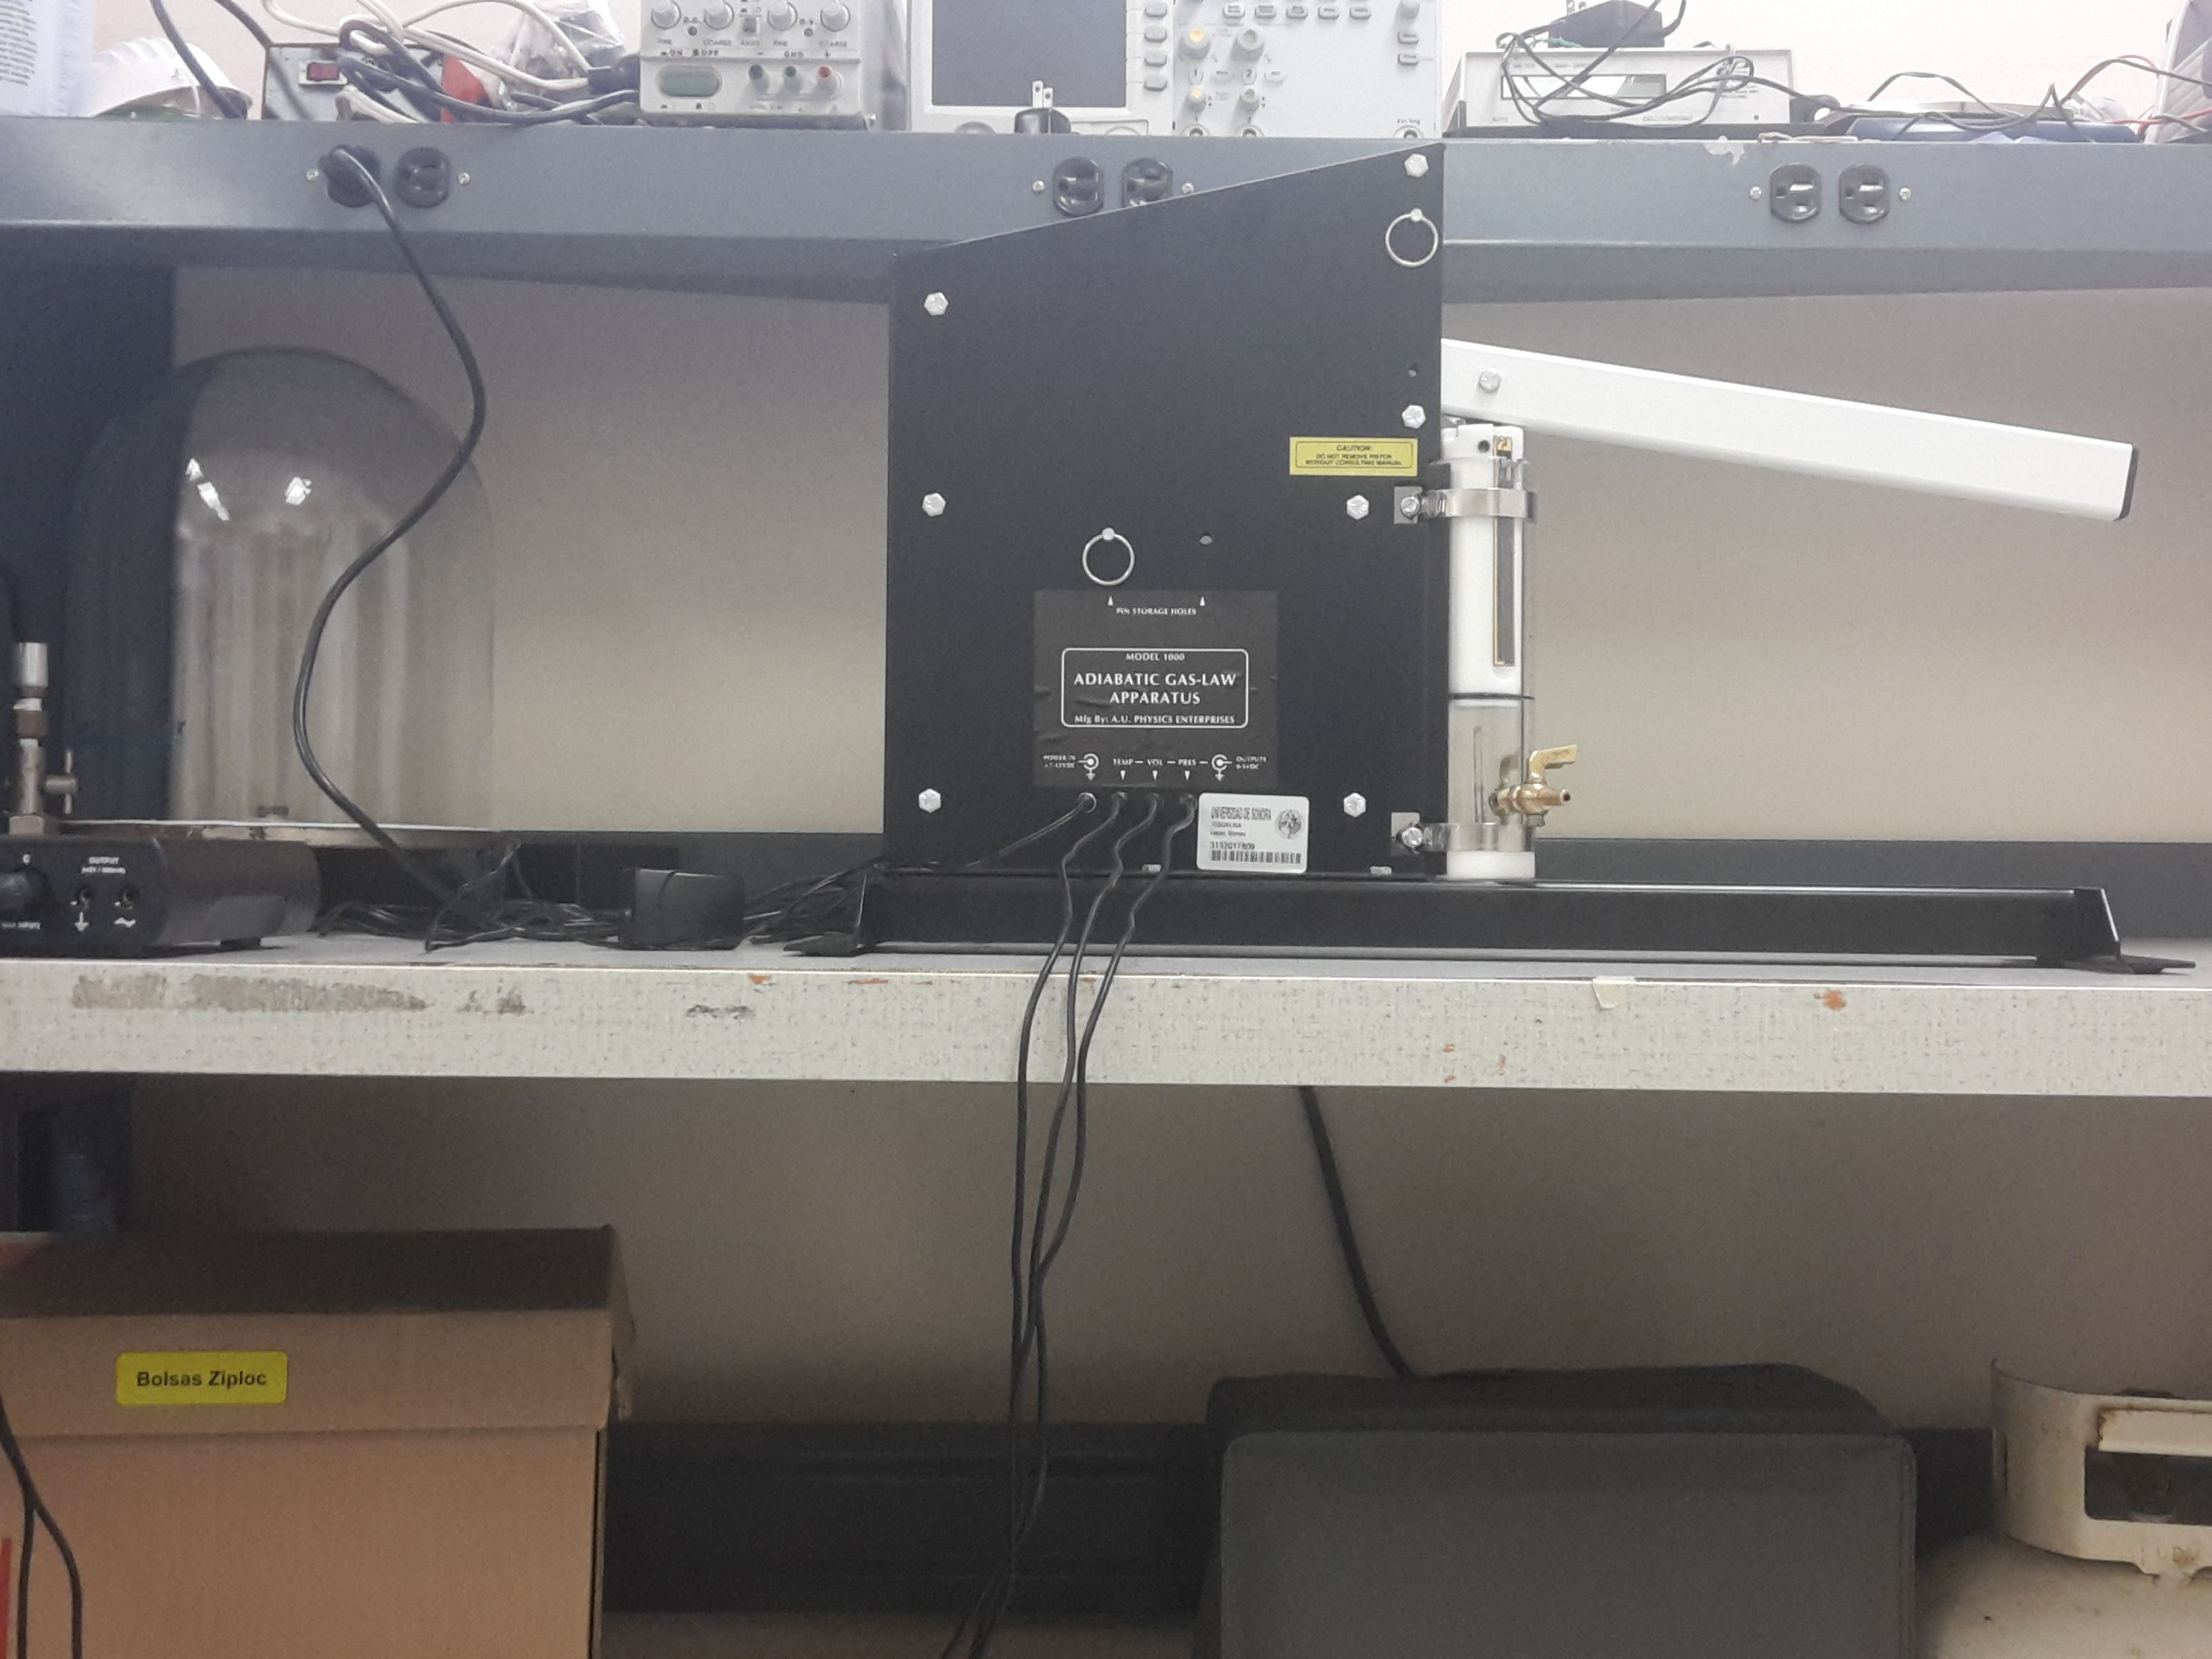
\includegraphics[width= 0.35\linewidth]{config.jpg}
 \caption{Arreglo experimental}
 \end{figure}
\pagebreak
%===================================================================================================
\section{Resultados}
La figura \ref{fig:Iso} muestra los resultados obtenidos del proceso lento.
\begin{figure}[H]
\centering
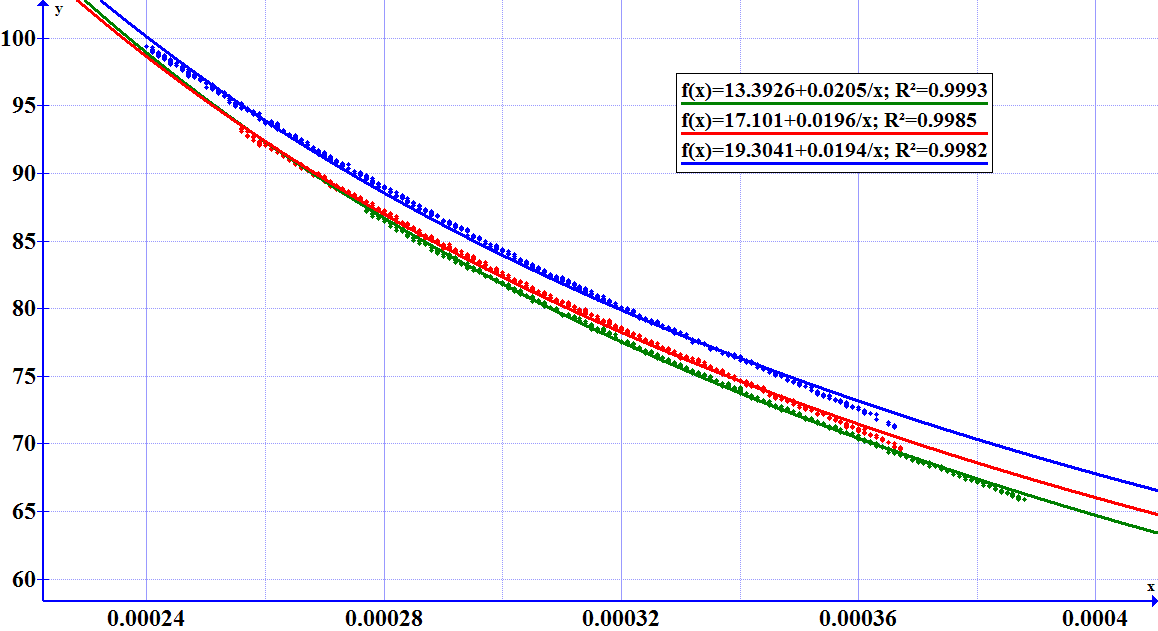
\includegraphics[width=0.75\linewidth]{Isoter.png}
\caption{Proceso lento con sus ajustes}
\label{fig:Iso}
\end{figure}
Recordando que fue un proceso de compresión, los puntos iniciales corresponden al volumen máximo y los puntos finales al volumen mínimo. Los ajuste para cada uno de los procesos se muestran en la figura \ref{fig:aIso}:
\begin{figure}[H]
\centering
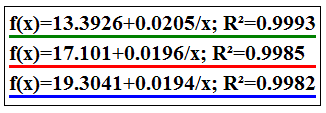
\includegraphics[width=0.35\linewidth]{AIsoter.png}
\caption{Ajustes del proceso lento}
\label{fig:aIso}
\end{figure}
\pagebreak
En caso del proceso rápido, les resultado se muestran en la figura \ref{fig:adb} 
\begin{figure}[H]
\centering
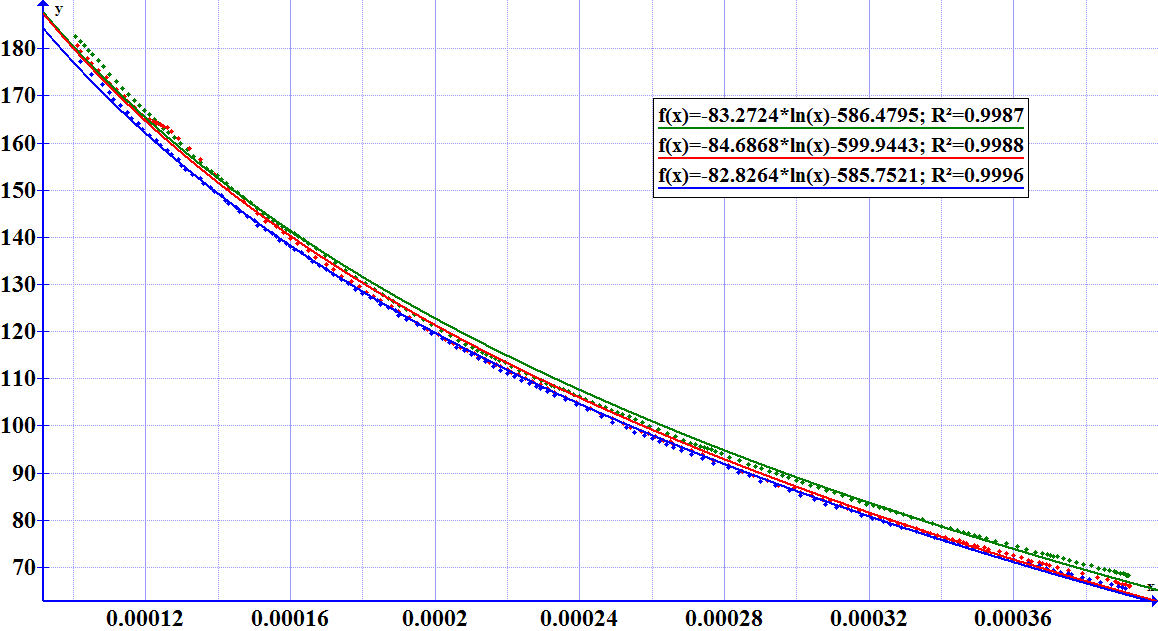
\includegraphics[width=0.75\linewidth]{Adiab.png}
\caption{Proceso rápido con sus ajustes}
\label{fig:adb}
\end{figure}
Recordando que fue un proceso de compresión, los puntos iniciales corresponden al volumen máximo y los puntos finales al volumen mínimo. Los ajuste para cada uno de los procesos se muestran en la figura \ref{fig:aadb}:

\begin{figure}[H]
\centering
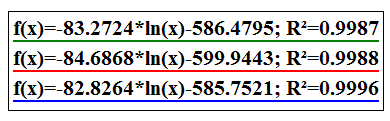
\includegraphics[width=0.35\linewidth]{AAdiab.png}
\caption{Ajustes del proceso Rápido}
\label{fig:aadb}
\end{figure}

Para obtener el área bajo la curva o trabajo termodinámico, se hizo uso del software con la que se realizaron los diagramas PV (Graph), el cual permite calcular la integral definida. La tabla \ref{tab:traIso} muestra el trabajo termodinámico realizado en los procesos lentos y la tabla \ref{tab:traAdb} los procesos rápido.

\begin{table}[H]
\centering
\begin{tabular}{|c|c|}
\hline
Proceso & Trabajo \\ \hline
1 & 8.40 J \\ \hline
2 & 8.94 J \\ \hline
3 & 10.61 J \\ \hline
\end{tabular}
\caption{Trabajo termodinámico realizado en los procesos lentos}
\label{tab:traIso}
\end{table}

\begin{table}[H]
\centering
\begin{tabular}{|c|c|}
\hline
Proceso & Trabajo \\ \hline
1 & 32.21 J \\ \hline
2 & 31.69 J \\ \hline
3 & 31.12 J \\ \hline
\end{tabular}
\caption{Trabajo termodinámico realizado en los procesos rápidos}
\label{tab:traAdb}
\end{table}
Los valores varían en esta magnitud debido a que no son el mismo proceso, ya que no se tienen la misma condiciones iniciales. Se puede observar que el trabajo es mayor en el proceso rápido que en el lento.

La ecuación de estado de un gas ideal esta dada por:
\begin{equation} \label{eq:ideal}
PV=nRT
\end{equation}
Si despejamos $n$ de \eqref{eq:ideal}, se obtiene el numero de moles del proceso. Si sutituimos con condiciones iniciales de los sistemas se obtiene:
$$n = \frac{PV}{RT} = 0.0107 moles$$
Con esto podemos comparar los resultados con los del gas ideal.

\textbf{Trabajo isotérmico de Gas Ideal}
$$W=nRT\ln\frac{V_f}{V_0}$$
\begin{table}[H]
\centering
\begin{tabular}{|c|c|c|c|}
\hline
Proceso & Experimental & Gas ideal& Error (\%) \\ \hline
1 & 8.40  J & 8.93  J & 5.94 \\ \hline
2 & 8.94  J & 9.03  J & 0.99 \\ \hline
3 & 10.61 J & 11.20 J & 5.27 \\ \hline
\end{tabular}
\caption{Comparación del Trabajo en procesos lentos}
\label{tab:traIsocomp}
\end{table}

\textbf{Trabajo adiabático de Gas Ideal}
$$ W = \frac{K(V_f^{1-\gamma}- V_0^{1-\gamma})}{1-\gamma} $$
donde $K =P_0V_0^\gamma $ y $\gamma =1.66$.

\begin{table}[H]
\centering
\begin{tabular}{|c|c|c|c|}
\hline
Proceso & Experimental & Gas ideal& Error (\%) \\ \hline
1 & 32.21 J & 58.76 J & 45.18 \\ \hline
2 & 31.69 J & 56.03 J & 43.45 \\ \hline
3 & 31.12 J & 55.39 J & 43.82 \\ \hline
\end{tabular}
\caption{Comparación del Trabajo en procesos rápidos}
\label{tab:traAdbcomp}
\end{table}


%===================================================================================================
\section{Discusión}
Lo que se observa en la tabla \ref{tab:traIsocomp} del proceso lento (isotérmico), fue que nuestros valores se parecen a nuestros valores teóricos, por lo que se puede decir es que tiene comportamiento de gas ideal para el proceso isotérmico.

Para el proceso rápido (adiabático), lo que muestra la tabla \ref{tab:traAdbcomp}, nuestros errores son muy grandes, lo que no lleva a pensar a que no tiene comportamiento de gas ideal.
%===================================================================================================
\section{Conclusiones}
En conclusión, esta experiencia de laboratorio, no llevo a encontrar que el proceso lento o isotermo tenia un comportamiento de gas ideal, mientras que el adiabático no dice lo contrario. Se llego a que el trabajo termodinámico se puede encontrar del área debajo de la curva en el diagrama PV.

 Los datos se pudieran mejorar si se usara un muestreo mas pequeño ya que había valores repetidos.  

%================================================================================================


\begin{thebibliography}{6}

\bibitem{a}
Universidad de Sevilla(s.f.) \textit{Trabajo en termodinámica} Recuperado de:
\url{http://laplace.us.es/wiki/index.php/Trabajo_en_termodin\%C3\%A1mica_(GIE)}

\bibitem{acu}
Acu\~na, H. (2015). \textit{Manual de Guías de Experiencias en el Laboratorio de Termodinámica Clásica}.

\end{thebibliography}
%================================================================================================

\end{document}

